\documentclass[a4paper, 11pt]{report}
\usepackage{times,epsfig,calc,subfigure}
\usepackage[authoryear,round]{natbib}
\usepackage{amsmath}
\usepackage{amsthm}
\usepackage{multicol}
%\usepackage[tablesfirst, nolists]{endfloat}
\usepackage{amsbsy, epsfig, epsf, psfrag, booktabs, graphicx, amssymb, enumerate}
\usepackage[hidelinks,bookmarks=false]{hyperref}
\usepackage{lscape}
\usepackage{bm}
\usepackage{float}
\floatplacement{table}{!htbp}
\usepackage{adjustbox}
\usepackage{color, colortbl}

\definecolor{Gray}{gray}{0.9}

\usepackage{makecell}
\usepackage{changepage}%adjust
\usepackage{setspace}%stretch
\usepackage{booktabs} 
\usepackage{multirow}
%\usepackage{hypernat}
\usepackage{authblk}
\usepackage{rotating}
\usepackage{multicol}
\usepackage{epstopdf}
\usepackage{tabularx, caption}
\usepackage[flushleft]{threeparttable}
\usepackage{grad}

\usepackage{kotex}
\usepackage{placeins}



\theoremstyle{definition}
\newtheorem{algo}{Algorithm}[section]



\makeatletter
\newcommand{\distas}[1]{\mathbin{\overset{#1}{\kern\z@\sim}}}%
\newsavebox{\mybox}\newsavebox{\mysim}
\newcommand{\distras}[1]{%
	\savebox{\mybox}{\hbox{\kern3pt$\scriptstyle#1$\kern3pt}}%
	\savebox{\mysim}{\hbox{$\sim$}}%
	\mathbin{\overset{#1}{\kern\z@\resizebox{\wd\mybox}{\ht\mysim}{$\sim$}}}%
}
\makeatother

\renewcommand{\baselinestretch}{1}
\linespread{1.4}
\renewcommand{\arraystretch}{1.3}
\newcommand{\cov}{\mathop{\rm cov}\nolimits} %covariance
\newtheorem{thm}{Theorem}[section]
\newtheorem{prop}[thm]{Proposition}
\newtheorem{defn}[thm]{Definition}
\newcommand\defeq{\mathrel{\overset{\makebox[0pt]{\mbox{\normalfont\tiny\sffamily def}}}{=}}}
\DeclareMathOperator*{\argmin}{argmin}

%%%%%%%%%%%%%%%%%%%%%%%
%   TITLE
%%%%%%%%%%%%%%%%%%%%%%%

\title{BSTERGMs: Bayesian Separable-Temporal Exponential family Graph Models}
\author{Seokjun Choi}
\date{December 2020}

\begin{document}	
\maketitle \pagestyle{plain}

\newpage
\thispagestyle{empty}

  \null
  \begin{center}
    \vskip -1.4cm
    {\fontsize{14pt}{14pt}\selectfont This certifies that Master's thesis of Seokjun Choi is approved.}
    \vskip 4cm%
    {\hskip 5cm\fontsize{12pt}{12pt}\selectfont \underline{\hskip 8cm}}\vspace*{0.2cm}\\
    \hskip 5cm\fontsize{12pt}{12pt}\selectfont Thesis Supervisor: Prof. Ick Hoon Jin\\
    \vskip 2cm
    {\hskip 5cm\fontsize{12pt}{12pt}\selectfont \underline{\hskip 8cm}}\vspace*{0.2cm}\\
    \hskip 5cm\fontsize{12pt}{12pt}\selectfont Committee Member: Prof. Chul Eung Kim\\
    \vskip 2cm
    {\hskip 5cm\fontsize{12pt}{12pt}\selectfont \underline{\hskip 8cm}}\vspace*{0.2cm}\\
    \hskip 5cm\fontsize{12pt}{12pt}\selectfont Committee Member: Prof. Jaewoo Park\\
    \vskip 3cm%
    {\fontsize{14pt}{14pt}\selectfont {The Graduate School \vskip 1.0em Yonsei University \vskip 1.0em Dec 2020}}%
  \end{center}
  \par
\clearpage

\pagestyle{plain}

\clearpage \pagenumbering{roman} \tableofcontents \clearpage

\clearpage \addcontentsline{toc}{chapter}{\protect\numberline{}
	\hspace*{-0.29in} List of Figures}
\listoffigures

\clearpage \addcontentsline{toc}{chapter}{\protect\numberline{}
    \hspace*{-0.29in} List of Tables}
\listoftables

\clearpage \addcontentsline{toc}{chapter}{\protect\numberline{}
    \hspace*{-0.29in} Abstracts}

%%%%%%%%%%%%
% ABSTRACT %
%%%%%%%%%%%%

\begin{abstract}
\begin{center}
{\LARGE 
BSTERGMs: The Bayesian Separable-Temporal Exponential family Graph Models
}
\end{center}
\indent
\vskip 0.8cm
\noindent
\vskip 0.2cm


The Separable Temporal Exponential Random Graph Models (STERGMs)(\cite{RN93}) are useful models to describe changes in dynamic networks' structures evolving over time. 
The Bayesian-inference based approach for the models, however, had not been developed yet. 
In this paper, I propose the Bayesian Separable Temporal Exponential Random Graph Models (BSTERGMs): STERGMs with the Bayesian setting, 
and illustrate a computational algorithm that generates posterior samples from the models dealing with the doubly-intractable constant problem. 
Furthermore, I show an inference method of the models in the Bayesian context.


\vspace{\stretch{1}} \noindent
\hrulefill\\
{\bf Key words}
\parbox[t]{0.8\textwidth}
{ : Networks, Exponential Random Graph Models, Bayesian inference, Marcov chain Monte Carlo, Longitudinal}
\end{abstract}

%--------------------------------------------------------------------------------%
%--------------------------------------------------------------------------------%
\clearpage
\chapter{Introduction} \label{Intro}
\pagenumbering{arabic}

Nowadays, new kinds of data with special forms emerge in many fields.
A sequence of real number values do not confine these new data as traditional data are in the past.
The data may have a non-number type of value, unique structure, or even integrated different types of values with model-specific relation.
These data are called complex data, and the attention of statistical analysis on the data increases over time.

As one form of complex data, network, or random graph gets highlighted attention as a flexible modeling tool for statistical analysis.
Many phenomena in the real world can be represented effectively by a form of networks. 
For example, social networks, including offline and online, can be thought of as networks.
Under an specific object of social science, some aspects of the relationship among actors 
can be modeled by networks, such as an analysis of power structure or a summary of intimacy structure on a given group. 
Another example is an application to a transmitted disease in epidemiology.
Modeling an infection using networks enables statistical analysis based on real data.

The ability to capture distinct features on an observed network enlarges statistical models' usefulness on networks. 
The statistical models give information about local relations like formation or dissolution between two actors 
as well as global features of the whole network, such as the probability that a specific structure realizes. 
The statistical models investigate the complex behavior of networks, 
including how the observed network's global features may be related to local network structure. 
During the investigation, the statistical models can capture existing dependency on a given network and provide a tool 
to understand what certain structural features are more common on rare.

Exponential-family random graph models(ERGMs) may be the most useful tools to analyze cross-sectional networks and their dependencies.
\cite{RN117}, \cite{RN123}, \cite{RN124} and \cite{RN122} proposed the models and apply them to analyze dependent structures, 
and \cite{RN115} and \cite{RN116} started the Bayesian approaches of the models.
In the ERGMs, the dependencies are captured by a series of local features called network statistics from classical graph theory. 
Since these models play an important role throughout this paper, I will introduce them more precisely in the following chapter.

The next natural question is a way to model a network sequence or network evolution over time. 
For instance, one may want to model social network structures for one year or 
simulate a disease infection based on the sequential observations in the past. 
The first exploration applying ERGMs to a network sequence was \cite{RN109}. 
After them, a notable contributions were of \cite{RN125} and \cite{RN126}, the Temporal ERGMs (TERGMs). 
In the TERGMs, the ERGMs are used by modeling the transition probability between times. 
Moreover, \cite{RN93} extend the TERGMs to the Separable Temporal ERGMs (STERGMs), 
considering the separation between duration - how long ties tend to last - and 
incidence - the rate at which new ties are formed - from 
prevalence - for example, the total number of ties - of the network properties. 
By imposing a conditional independence condition between the duration and incidence on the model, 
the models can be extended to more effectively interpretable ones than the TERGMs 
without adding much complexity.

Although the STERGMs give us strength when interpreting the fitted parameter, 
a Bayesian approach for the STERGMs has not been conducted. 
It is partly because of the hardship from the massive computation in the parameter estimation method for the models. 
Nonetheless, the Bayesian approach of STERGMs provides the statistical inference method following the standard Bayesian way, 
so the approach has a huge advantage of convenience for statistical works for fitted parameters and predictions to next time network structure. 
Thus, in this paper, I specify the Bayesian separable temporal exponential random graph models (BSTERGMs) and propose a fitting algorithm for the model parameters.
I also discuss the inference methods, the diagnostics and goodness of fit checking procedures.

Chapter 2 reviews the background materials, including the ERGMs, the BERGMs, the TERGMs, and the STERGMs. 
In chapter 3, I propose the BSTERGMs and show the detailed setting of BSTERGMs. 
In the following chapter, chapter 4, I offer the estimation method for the BSTERGMs. 
Chapter 5 explains ways to conduct diagnostics, statistical inference, and goodness of fit checks. 
Besides, I illustrate an application of BSTERGMs to network data of scholars and faculty
from the UCLA medical working project team in chapter 6, 
Finally, in chapter 7, I discuss some possible extensions and ways to supplement the BSTERGMs further for future research.

%--------------------------------------------------------------------------------%
%--------------------------------------------------------------------------------%


\chapter{Background} \label{Chapter2}
\section{Random graphs}
Networks or random graphs play a central role as a general model 
describing relations among subjects in the statistical context. 
To begin with, I briefly summarize some terminologies and notations for concepts related to the networks.

In this paper, I will use two words, 'graphs' and 'network,' as the same meaning without distinction.
We say each subject on the data to a node. 
They sometimes are called vertex in graph theory. 
In addition, we say a tie joining two nodes to an edge. A tie can be directed or not. 
These two components have a fundamental role in describing the relational structure. 
Define a graph or a network to $y=(V,E)$, where $V$ is a set of nodes, and $E$ is a set of edges of a network.

For simplicity, I will deal with a situation without weights on each node or edge.
Then, a graph $y$ can be represented by a more straightforward form.
Assume that the number of node $n\in \mathbb{N}$ on data is given.
Then, for $\mathcal{B}=\{0,1\}$,
a set $\mathcal{Y} \subset \mathcal{B}^{n^2}$ is a set of graphs of $n$ nodes.
Now, a graph $y \in \mathcal{Y}$ can be represented by a $n \times n$ binary matrix
with elements $y_{ij}=1$ if there is a tie from $i$-th node to $j$-th node,
otherwise $y_{ij}=0$.

If edges of $y$ have directions, then $y$ is called a directed graph. Otherwise, $y$ is called an undirected graph.
These are obvious that, for given $n\in \mathbb{N}$,
$|\mathcal{Y}|=2^{n(n-1)}$ if $\mathcal{Y}$ is the set of all directed graphs not permitting self-connecting edges,
and $|\mathcal{Y}|=2^{n(n-1)/2}$ if $\mathcal{Y}$ is the set of all graphs of undirected one.
Thus, the size of $\mathcal{Y}$ exponentially grows when n increases.

I extend the concept of graphs to describe a situation that connections among nodes are random.
Let $\Omega$ be an event set of all possible connected situations among given nodes.
We say $Y: \Omega \to \mathcal{Y}$ is a random variable for a graph, or a random graph.
For a random graph $Y$, denote the edge between i-th node and j-th node by $Y_{ij}$ for $i,j=1,2,...,n$
satisfying $Y_{ij}=1$ if the edge is connected. Otherwise, $Y_{ij}=0$.
Note that the $Y_{ij}$s are also random variables in our context.

Let me notate a realization of random graph by $y$ and its edges by $y_{ij}$ for $i,j=1,2,...,n$.


\section{ERGMs: Exponential random graph models}
One of the natural questions from the definition of the random graphs is 
how we can model a probability distribution to the graphs.
As a answer, the Exponential random graph models (ERGMs) (\cite{RN123} and \cite{RN122})
gives a classical but flexible scheme to model for time-invariant networks represented as a single directed or undirected graph.
Moreover, the ERGMs provide a statistical approach to the systematic exploration of several local features simultaneously and 
how these local structures interact to form a global network.

Specifically, following the notation of the previous section,
let $\mathcal{Y}$ be a set of networks with $n$ nodes and $Y$ be a random graph.
Set a distribution of $Y$ to
    \[P(Y=y;\theta) = \frac{exp(\theta^{T}s(y))}{c(\theta)}\]
for some $\theta\in\mathbb{R}^p$,
where $s(y)\in\mathbb{R}^p$ is a vector which is part of sufficient network statistics of $y\in\mathcal{Y}$,
and $c(\theta)\in\mathbb{R}$ is a normalizing constant satisfying $c(\theta)=\sum_{y\in\mathcal{Y}}exp(\theta^{T}s(y))$.
Models that have such a form are called the ERGMs.

Note that the form of the right-hand side is a canonical form of exponential family distributions.
That is why the model is called exponential. 
Although the form is familiar, directly calculating the normalizing constant is not possible in practical data analysis 
because the size of $\mathcal{Y}$ grows exponentially as $n$ grows. 
Thus for the application to the real data, the calculation of $c(\theta)$ should be avoided.
Luckily, some fitting algorithms have been developed for this issue. 
If you need, see \cite{RN100} addressing the ergm package in R with the MCMCMLE or the classic method using pseudolikelihood. 
For more detail of the MCMCMLE algorithm, see \cite{RN104}


\section{BERGMs: Bayesian ERGMs}
\cite{RN115} and \cite{RN116} extend ERGMs to bayesian setting. 
Putting prior $p(\theta)$ to the parameter $\theta$, the model becomes
\[p(\theta|y)=\frac{p(y|\theta)p(\theta)}{p(y)}=\frac{exp(\theta^T s(y))}{c(\theta)}\frac{p(\theta)}{p(y)}\]

Observe that not only $c(\theta)$ but also the $p(y)$ cannot be evaluated directly
because of the difficulty of summation when $n$ grows and of integration of $p(y)$.
Moreover, the constant depends on the parameter $\theta$, so the ordinary MCMC technique cannot be used.
This situation is said to the doubly intractable constant problem(\cite{RN119}), 
and causes a serious challenge to estimate the parameter vector $\theta$.
Thus, The estimation of $\theta$ needs an advanced algorithm than the standard MCMC procedure.
The solution of Caimo and Friel is using the exchange algorithm. 
You can see \cite{RN115} for details of fitting methods of BERGMs
and \cite{RN127} for the exchange algorithm.


\section{TERGMs: Temporal Exponential family Random Graphs Models}
Let's consider a sequence of random graph $\{Y_1, Y_2, ..., Y_T\} (T\in\mathbb{N})$ and assume that
we are interested in the dynamics or evolution of the network sequence.
The Temporal Exponential family Random Graphs Models(TERGMs)
proposed by \cite{RN125} and \cite{RN126}
are models for our interest if we permit a Markov assumption
\[P(Y_2,Y_3,...,Y_T|Y_1)=P(Y_2|Y_1)P(Y_3|Y_2)...P(Y_T|Y_{T-1})\]
and focus on the transition probability along index of the sequence.
For convenience, I refer to the index $1,2,...,T$ as a time.

Specifically, let $\mathcal{Y}$ be a set of graphs with $n$ nodes. 
Let $Y_1=y_1 \in \mathcal{Y}$ be given and $Y_2,...,Y_T (T\in\mathbb{N})$ be random graphs.
Set a distribution of $Y_2,...,Y_T$ by
\[P(Y_t=y_t|Y_{t-1}=y_{t-1};\theta) = \frac{exp(\theta^{T}s(y_t, y_{t-1}))}{c(\theta, y_{t-1})}\]
where $t=2,...,T$, $y_t\in\mathcal{Y}$, $\theta\in\mathbb{R}^p$,
sufficient network statistics $s(y_t, y_{t-1})\in\mathbb{R}^n$,
and a normalizing constant $c(\theta, y_{t-1})=\sum_{y\in\mathcal{Y}}exp(\theta^{T}s(y, y_{t-1}))$.
Models that have such a form are called the TERGMs.

The estimation of $\theta$ can be performed by MCMCMLE.
Nevertheless, the estimation suffers severe degeneracy problem.
Furthermore, When interpreting the estimated TERGMs parameters,
we cannot separate the generation and duration because
the parameter value of $\theta$ affects both.
These raise demand for modified models to remedy the degeneracy and enable separable interpretation.

\section{STERGMs: Separable-Temporal Exponential family Random Graphs Models}
One solution to remedy the problems of TERGMs is 
the Separable-Temporal Exponential family Random Graphs Models, or simply STERGMs (\cite{RN93}.)
The key idea is to separate the formation models and dissolution model
for decoupling an effect on edge's duration of the model parameter from edge's incidence
when setting a distribution on a sequence of random graph.

Precisely,
let $\mathcal{Y}$ is a set of graphs with given $n\in\mathbb{N}$ nodes. 
Suppose $Y_1=y_1 \in \mathcal{Y}$ be given and $Y_2,...,Y_T (T\in\mathbb{N})$ be random graphs.
Let $\mathcal{Y}^+|_t$ be a subset of $\mathcal{Y}$ consisting of all graphs which have equal or additional edges comparing to $y_{t-1}$.
Likewise, let $\mathcal{Y}^-|_t$ be a subset of $\mathcal{Y}$ consisting all graphs which have equal or sparse edges comparing to $y_{t-1}$.
Next, for random graphs $Y_t^+: \Omega \to\mathcal{Y}^+|_t$, $Y_t^-: \Omega \to\mathcal{Y}^-|_t$,
and graphs $y_t^+ \in \mathcal{Y}^+|_t$, $y_t^- \in \mathcal{Y}^-|_t$, set
\[P(Y_t^+=y_t^+|Y_{t-1}=y_{t-1};\theta^+) = \frac{exp((\theta^+)^{T}s(y_t^+, y_{t-1}))}{c(\theta^+, y_{t-1})}\]
\[P(Y_t^-=y_t^-|Y_{t-1}=y_{t-1};\theta^-) = \frac{exp((\theta^-)^{T}s(y_t^-, y_{t-1}))}{c(\theta^-, y_{t-1})}\]
for parameters $\theta^+,\theta^-\in\mathbb{R}^p$, parts of sufficient network statistics $s(y_t^+, y_{t-1}), s(y_t^-, y_{t-1})\in\mathbb{R}^p$,
and normalizers $c(\theta^+, y_{t-1})=\sum_{y^+\in\mathcal{Y}^+}exp((\theta^+)^{T}s(y^+, y_{t-1}))$, 
$c(\theta^-, y_{t-1})=\sum_{y^-\in\mathcal{Y}^-}exp((\theta^-)^{T}s(y^-, y_{t-1}))$.

Then, defining operations $+,-$ on $\mathcal{Y}$ following the edgewise boolean algebra,
(For detail, Define binary operations on the edge values $\{0,1\}$ by $+$ and $-$ 
by $1+1=1, 1+0=0+1=1, 0+0=0$ and $1-1=0, 1-0=1, 0-1=0, 0-0=0$) 
and set the combined network $y_t$ to
\[y_t=y_t^+ - (y_{t-1} - y_t^-) = y_t^- + (y_t^+ - y_{t-1})\]

Additionally, assume the first-order Markov assumption,
\[P(Y_2,...,Y_T|Y_1)=P(Y_2|Y_1)...P(Y_T|Y_{T-1})\]
and the conditional independence between $Y_t^+$ and $Y_t^-$ for all $t=2,...,T$.
Note that the last condition is called the separability.
Then we get
\begin{multline}
    P(Y_t=y_t|Y_{t-1}=y_{t-1};\theta^+,\theta^-) \\
    = P(Y_t^+=y_t^+|Y_{t-1}=y_{t-1};\theta^+) P(Y_t^-=y_t^-|Y_{t-1}=y_{t-1};\theta^-)
\end{multline}
Models that have such a form are called the STERGMs.



\section{Network Statistics for ERGMs and derived models}
Now, I briefly discuss the terms of network statistics.
As a usual, $s(y)$ of ERGMs or $s(y_{t}^.,y_{t-1})$ of TERGMs and STERGMs would 
reflect the structure of given network without identifying each node index.
Typical candidates are here.


Let $y\in\mathcal{Y}$ and $n\in\mathbb{N}$ be the number of nodes of $y$.
The most straightforward candidate is the number of edges, denoted by $|y|$.

Following \cite{RN104}, usual candidates are distributions defined by some sense of the structure of a given graph. 
For a given $i, 1\leq i \leq n-1$, $D_i(y)$ is defined as the number of nodes in y whose the number of edges incident to the node equals $i$, 
and called the $i$-th order node degree distribution. 

For a given $i, 1\leq i \leq n-2$, $P_i(y)$ is defined to be the number of dyads $(j,k), 1\leq j,k \leq n$
in y whose $j$ and $k$ have nodes connected by an edge each other and they share exactly $i$ connected nodes in common,
and called the $i$-th order edgewise shared partner distribution.

Note that the bundle of all order of the node degree distribution and all order of the edgewise shared partner distribution,
\[(D_1(y),D_2(y),...,D_{n-1}(y),P_1(y),P_2(y),...,P_{n-2}(y))\] 
forms sufficient statistics of a graph.
Moreover, there are relation that
\[n=D_0(y)+D_1(y)+...+D_{n-1}(y)\]
and
\[|y|=P_0(y)+P_1(y)+...+P_{n-2}(y)=\frac{1}{2}\sum_{i=1}^{n-1} iD_i(y)\]


A function of the sufficient statistics can be candidates for the model statistics.
\cite{RN128} proposed graph statistics including the $k$-star $S_k(y)$ for $1\leq k \leq n-1$ and the $k$-triangles $T_k$ for $1\leq k \leq n-2$.
The $k$-star consists of a node together with a set of $k$ of its connected nodes.
The $k$-triangle consists of $k$ triangles that share one common edge.
They can be expressed by the definition of node degree distributions and edgewise shared partner distributions,
\[S_1 = |y|, 
S_k = \sum_{i=1}^{n-1} \binom{i}{k} D_i(y), k\geq 2\]
and
\[T_1 = \frac{1}{3}\sum_{i=1}^{n-2} iP_i(y),
T_k = \sum_{i=1}^{n-2} \binom{i}{k} P_i(y), k\geq 2\]

Another interesting statistics are the geometrically weighted value of distributions defined by
\cite{RN118}, \cite{RN104}, \cite{RN128} and \cite{RN103}.
For example, the geometrically weighted (node) degree with parameter $\tau$ is defined by
\[GWD(y;\tau)=e^{\tau} \sum_{k=1}^{n-2} (1-(1-e^{-\tau})^k)D_k(y)\]
and the geometrically weighted shared partner distribution with parameter $\tau$ is defined by
\[GWESP(y;\tau)=e^{\tau} \sum_{k=1}^{n-2} (1-(1-e^{-\tau})^k)P_k(y)\]


In the context of temporal models, parameters in the model take two network as a arguments like $s(y_t,y_{t-1})$.
One of the common choices for these statistics is the bundle of sufficient statistics of first argument $y_t$.
Another common choice is using a difference, $s(y_t,y_{t-1})=s'(y_t)-s'(y_{t-1})$ where $s'$ is a network statistics of given network.
Although there are many other statistics related to the ERGMs, I omit them and end this section here.
For additional example, see \cite{RN107} for the ERGMs, and \cite{RN125}'s chapter 2.1 for the TERGMs.




%--------------------------------------------------------------------------------%
%--------------------------------------------------------------------------------%
\chapter{Bayesian STERGMs} \label{Cahpter3}

The goal of this chapter is to convert the STERGMs to the Bayesian setting.
With priors $p(\theta^+),p(\theta^-)$ over $\theta^+,\theta^-$,
the Bayesian model for the STERGMs can be made. I call this model the Bayesian Separable Temporal Exponential family Random Graph Models,
or the BSTERGMs. 

More explicitly, let $\mathcal{Y}$ be the set of all networks with $n\in \mathbb{N}$ nodes. Let $Y_1=y_1 \in \mathcal{Y}$ be given and $Y_2,...,Y_T, T\in\mathbb{N}$ be random graphs.
As the STERGMs, define $\mathcal{Y}^+|_t$, $\mathcal{Y}^-|_t$ be subsets of $\mathcal{Y}$ consisting all graphs which have equal or additional edges comparing to $y_{t-1}$,
and which have equal or sparse edges comparing to $y_{t-1}$, respectively.
Then, for random graphs $Y_t^+: \Omega \to \mathcal{Y}^+|_t$, $Y_t^-: \Omega \to \mathcal{Y}^-|_t$,
and graphs $y_t^+ \in \mathcal{Y}^+|_t$, $y_t^- \in \mathcal{Y}^-|_t$, set formation model
\[P(Y_t^+=y_t^+|Y_{t-1}=y_{t-1};\theta^+) = \frac{exp((\theta^+)^{T}s(y_t^+, y_{t-1}))}{c(\theta^+, y_{t-1})}\]
and dissolution model
\[P(Y_t^-=y_t^-|Y_{t-1}=y_{t-1};\theta^-) = \frac{exp((\theta^-)^{T}s(y_t^-, y_{t-1}))}{c(\theta^-, y_{t-1})}\]
for parameters $\theta^+,\theta^-\in\mathbb{R}^p$, network statistics $s(y_t^+, y_{t-1}), s(y_t^-, y_{t-1})\in\mathbb{R}^p$,
and normalizers 
\[c(\theta^+, y_{t-1})=\sum_{y^+\in\mathcal{Y}^+}exp((\theta^+)^{T}s(y^+, y_{t-1}))\]
\[c(\theta^-, y_{t-1})=\sum_{y^-\in\mathcal{Y}^-}exp((\theta^-)^{T}s(y^-, y_{t-1}))\]

Then, with the edgewise boolean algebra defined in chapter 2.5, set the combined network $y_t$ to
\[y_t=y_t^+ - (y_{t-1} - y_t^-) = y_t^- + (y_t^+ - y_{t-1})\]

and assume that the first-order Markov property
\[P(Y_2,...,Y_T|Y_1)=P(Y_2|Y_1)...P(Y_T|Y_{T-1})\]
and separability (or, conditional independence) between $Y_t^+$ and $Y_t^-$ for all $t=2,...,T$.

Then we get
\[\theta^+ \sim p(\theta^+)\]
\[\theta^- \sim p(\theta^-)\]
and
\begin{multline}
    P(Y_t=y_t|Y_{t-1}=y_{t-1};\theta^+,\theta^-) \\ 
    =P(Y_t^+=y_t^+|Y_{t-1}=y_{t-1};\theta^+) P(Y_t^-=y_t^-|Y_{t-1}=y_{t-1};\theta^-)
\end{multline}

The purpose of Bayesian inference is to get information of the posterior distribution of $\theta^+,\theta^-$.
By the Bayes rule, the posterior can be expressed by
\[P(\theta^+,\theta^-|y_t, y_{t-1}) = \frac{P(Y_t^+=y_t^+|y_{t-1},\theta^+) P(Y_t^-=y_t^-|y_{t-1},\theta^-)P(\theta^+),P(\theta^-)}{c(\theta^+,y_{t-1})c(\theta^-,y_{t-1})p(y_t, y_{t-1})} \]
where $y_t=y_t^+ - (y_{t-1} - y_t^-) = y_t^- + (y_t^+ - y_{t-1})$ as set above.
I define models that have such forms as the BSTERGMs.

Note that the BSTERGMs also have similar kinds of problems to the BERGMs.
The normalizing constants $c(\theta^+,y_{t-1})$, $c(\theta^-,y_{t-1})$ practically cannot be computed 
because there are too many terms to sum up.
The normalizing constants are doubly intractable since they depend on $\theta^+$ and $\theta^-$, the parameters of a model.
Thus, we cannot use a standard MCMC algorithm to get the posterior sample of the parameters
because the constant part remains when calculating the MCMC ratio.
I will address this issue with more details in the next chapter.


%--------------------------------------------------------------------------------%
%--------------------------------------------------------------------------------%
\chapter{Estimation} \label{Chapter4}

Suppose that a sequence of graphs $y_1,...,y_T$ in $\mathcal{Y}$ is observed.
(then, $y_2^+,...,y_T^+$ and $y_2^-,...,y_T^-$ are uniquely determined.) 
Then how can we find the posterior distribution of $\theta^+,\theta^-$ with the observation using the BSTERGMs?
In this chapter, I propose a novel algorithm to estimate parameters of the BSTERGMs using the exchange algorithm, 
one of the special MCMC techniques by \cite{RN127}.

The motivation of using the exchange algorithm comes from the algorithm of the BERGMs' (\cite{RN115})
to solve the doubly intractable constant problem. By extending the algorithm of the BERGMs,
I build the fitting algorithm for the BSTERGMs.
Although an approach using MCMC cannot give an analytic expression of the posterior distribution, 
it gives posterior samples as much as we want, so we can conduct statistical inference on given data using the generated samples.

Before introducing the new algorithm,
let us consider the ordinary MCMC ratio for $m$-th MCMC iteration in the BSTERGMs context
to show the doubly intractable constant problem explicitly.

For convenience, let the parameters of formation model and dissolution model are in $\mathbb{R}$.
With symmetric proposal distribution,
\[\pi_{ordinary} = \frac{P(y_t^+|y_{t-1},\theta_*^+)P(y_t^-|y_{t-1},\theta_*^-)p(\theta_*^+)p(\theta_*^-)}
{P(y_t^+|y_{t-1},\theta_{m-1}^+)P(y_t^-|y_{t-1},\theta_{m-1}^-)p(\theta_{m-1}^+)p(\theta_{m-1}^-)}\]
where $\theta^*$ is proposed parameter in an iteration of MCMC.
Plugging the model form,
\[\pi_{ordinary} = \frac{\frac{exp(\theta_*^+ s(y_t^+,y_{t-1}))}{c(\theta_*^+, y_{t-1})} \frac{exp(\theta_*^- s(y_t^-, y_{t-1}))}{c(\theta_*^-, y_{t-1})} p(\theta_*^+)p(\theta_*^-)}
    {\frac{exp(\theta_{m-1}^+ s(y_t^+, y_{t-1}))}{c(\theta_{m-1}^+, y_{t-1})} \frac{exp(\theta_{m-1}^- s(y_t^-, y_{t-1}))}{c(\theta_{m-1}^-,y_{t-1})} p(\theta_{m-1}^+)p(\theta_{m-1}^-)}\]
Since each c depends on unique subscript of $\theta$ respectively, the constants are not canceled out.

The key idea of new algorithm to solve this problem is running two MCMC chains to draw independent samples to cancel the constant parts
when calculating the MCMC accept-reject ratio. If we can generate simulated samples $y_{ex}|y_{t-1},\theta_{m-1}$ and $y_{ex}|y_{t-1},\theta_*$ and
consider their probability following the BSTERGMs, this situation can be resolved.
By multiplying the probability terms in order to exclude the constant terms,
we get the exchange algorithm's ratio,


\begin{equation}
    \begin{aligned}
        \pi & = \frac{P(y_t^+|y_{t-1},\theta_*^+)P(y_t^-|y_{t-1},\theta_*^-)p(\theta_*^+)p(\theta_*^-)P(y_{ex}^+|y_{t-1},\theta_{m-1}^+)P(y_{ex}^-|y_{t-1},\theta_{m-1}^-)}
        {P(y_t^+|y_{t-1},\theta_{m-1}^+)P(y_t^-|y_{t-1},\theta_{m-1}^-)p(\theta_{m-1}^+)p(\theta_{m-1}^-)P(y_{ex}^+|y_{t-1},\theta_*^+)P(y_{ex}^-|y_{t-1},\theta_*^-)} \\
        & = \frac{\frac{exp(\theta_*^+ s(y_t^+,y_{t-1}))}{c(\theta_*^+, y_{t-1})} \frac{exp(\theta_*^- s(y_t^-, y_{t-1}))}{c(\theta_*^-, y_{t-1})} p(\theta_*^+)p(\theta_*^-)}
        {\frac{exp(\theta_{m-1}^+ s(y_t^+, y_{t-1}))}{c(\theta_{m-1}^+, y_{t-1})} \frac{exp(\theta_{m-1}^- s(y_t^-, y_{t-1}))}{c(\theta_{m-1}^-,y_{t-1})} p(\theta_{m-1}^+)p(\theta_{m-1}^-)}
        \frac{\frac{exp(\theta_{m-1}^+)s(y_{ex}^+,y_{t-1})}{c(\theta_{m-1}^+, y_{t-1})}\frac{exp(\theta_{m-1}^- s(y_{ex}^-,y_{t-1}))}{c(\theta_{m-1}^-, y_{t-1})}}
        {\frac{exp(\theta_*^+ s(y_{ex}^+,y_{t-1}))}{c(\theta_*^+,y_{t-1})} \frac{exp(\theta_*^- s(y_{ex}^-,y_{t-1}))}{c(\theta_*^-,y_{t-1})}} \\
        & = \frac{exp(\theta_*^+ s(y_t^+,y_{t-1})) exp(\theta_*^- s(y_t^-, y_{t-1}))}{exp(\theta_{m-1}^+ s(y_t^+, y_{t-1}))exp(\theta_{m-1}^- s(y_t^-, y_{t-1}))}
        \frac{exp(\theta_{m-1}^+ s(y_t^+, y_{t-1}))exp(\theta_{m-1}^- s(y_{ex}^-,y_{t-1}))}{exp(\theta_*^+ s(y_{ex}^+,y_{t-1}))exp(\theta_*^- s(y_{ex}^-,y_{t-1}))} \\
        & \quad * \frac{p(\theta_*^+)p(\theta_*^-)}{p(\theta_{m-1}^+)p(\theta_{m-1}^-)} \\
        & = exp((\theta_*^+ - \theta_{m-1}^+)(s(y_t^+,y_{t-1}) - s(y_{ex}^+,y_{t-1}))(\theta_*^- - \theta_{m-1}^-)(s(y_t^-,y_{t-1}) - s(y_{ex}^-,y_{t-1}))) \\
        & \quad * \frac{p(\theta_*^+)p(\theta_*^-)}{p(\theta_{m-1}^+)p(\theta_{m-1}^-)}
    \end{aligned}
  \end{equation}


% \[=exp((\theta_*^+ - \theta_{m-1}^+)s(y_t^+,y_{t-1}) + (\theta_*^- - \theta_{m-1}^-)s(y_t^-,y_{t-1})
% -(\theta_*^+ - \theta_{m-1}^+)s(y_{ex}^+,y_{t-1}) - (\theta_*^- - \theta_{m-1}^-)s(y_{ex}^-,y_{t-1}))
% \frac{p(\theta_*^+)p(\theta_*^-)}{p(\theta_{m-1}^+)p(\theta_{m-1}^-)}\]



The last expression has no constant term depending on the parameters.
This result leads us to the fitting algorithm for the BSTERGMs using the exchange algorithm.

\clearpage
\begin{algo}[the main chain]
Let $y_1,...,y_T$ be given. For $m=1,...,M$,
\begin{enumerate}
    \item Propose candidates $\theta_*^+,\theta_*^-$ from a proposal distribution $\epsilon(.|\theta_{m-1}^+,\theta_{m-1}^-)$.
    \item Select a lag $(t-1,t)$ randomly on $2 \leq t \leq T$.
    \item Generate an exchange graph $y_{ex} \in\mathcal{Y}|_t$ (with $y_{ex}^+, y_{ex}^-$) at the $\theta_*^+,\theta_*^-$.
    \item Calculate network statistics $s(y_t^+,y_{t-1}), s(y_{ex}^+,y_{t-1}), s(y_t^-,y_{t-1}), s(y_{ex}^-,y_{t-1})$.
    \item Calculate the exchange MCMC ratio $\pi$ at the lag,
        \[\pi = \frac{P(y_t^+|y_{t-1},\theta_*^+)P(y_t^-|y_{t-1},\theta_*^-)p(\theta_*^+)p(\theta_*^-)\epsilon(\theta_{m-1}|\theta_*)}
            {P(y_t^+|y_{t-1},\theta_{m-1}^+)P(y_t^-|y_{t-1},\theta_{m-1}^-)p(\theta_{m-1}^+)p(\theta_{m-1}^-)\epsilon(\theta_*|\theta_{m-1})} \]
        \[* \frac{P(y_{ex}^+|y_{t-1},\theta_{m-1}^+)P(y_{ex}^-|y_{t-1},\theta_{m-1}^-)}{P(y_{ex}^+|y_{t-1},\theta_*^+)P(y_{ex}^-|y_{t-1},\theta_*^-)}\]
    \item With probability $min(\pi,1)$, accept the proposal and put $(\theta_m^+,\theta_m^-) = (\theta_*^+,\theta_*^-)$.\\
        Otherwise, reject the proposal and put $(\theta_m^+,\theta_m^-) = (\theta_{m-1}^+,\theta_{m-1}^-)$.
\end{enumerate}
\end{algo}    

For step 5, you can use the result of equation (4.1). If $s(.,.)$ and $\theta$ are multi-dimension (in $\mathbb{R}^p, p>1$,) 
replace the multiplications between $\theta$ and $s$ in the exponent parts to the dot product between two vectors.
In addition, when implementing the algorithm, I strongly recommend to use $log\pi$ instead of $\pi$ to avoid an underflow problem.

To get the exchange network $y_{ex}$ for time $t$ in the second part of the main chain, 
we need a generative algorithm at a given parameter points. 
However, since the normalizing constant is still unknown, 
we cannot get the generative algorithm directly using the model's expression. 
Thus, I use one more MCMC chain.

\begin{algo}[the auxiliary chain]
Let $\theta^+,\theta^-,y_{t-1}$ be given. For $k=1,...,K$,
\begin{enumerate}
    \item Select one edge randomly from the $y_{k-1}$, say, $y_{k-1;ij}$.
    \item Propose a new graph $y_*$ with switching the $y_{ij}$ value from $y_{k-1}$: 
    \\ If $y_{k-1;ij}=1$, then set $y_{*;ij}=0$ (dissolution case.) 
    \\ Otherwise, If $y_{k-1;ij}=0$, then set $y_{*;ij}=1$ (formation case.)
    \\ (If sample graphs are undirected, switch $y_{ji}$ simultaneously.)
    \item Take $\theta$ as $\theta^+$ or $\theta^-$ according to the case. Calculate the MCMC ratio $\phi$,
    \[\phi = \frac{P(Y_t=y_*|y_{t-1},\theta)}{P(Y_t=y_{k-1}|y_{t-1},\theta)}= exp(\theta^T (s(y_{*},y_{t-1}) - s(y_{k-1},y_{t-1})))\]
    \item With probability $min(\phi,1)$, accept the proposal and put $y_k=y_*$.\\
        Otherwise, reject the proposal and put $y_k=y_{k-1}$.
\end{enumerate}
\end{algo}

After $K$ iteration, use the last sample as the exchange sample in the second part of the main algorithm.



%--------------------------------------------------------------------------------%
%--------------------------------------------------------------------------------%
\chapter{Diagnostics, inference, and the Bayesian GOF} \label{Chapter5}

\section{Model diagnostics}
The ERGMs and all derived models of the ERGMs suffer the degeneracy problem: 
all exchange samples' nodes become fully connected or totally isolated as the MCMC chain runs. 
A degenerated chain may cause an explosion of estimated parameter to $\infty$ or $-\infty$,
failing to converge of MCMC chains. In fact, the BSTERGMs are no exception. 
Thus, the diagnostic process is a very important part of using the BSTERGMs.

Since two MCMC chains run in the fitting algorithm of the BSTERGMs, two diagnostic tasks should proceed.

The main chain produces the posterior samples of parameter
$\{\theta_i^+\}_{i=1}^M, \{\theta_i^-\}_{i=1}^M$ in $\mathbb{R}^p, p\in\mathbb{N}$,
so the diagnostic procedure is not different with an ordinary MCMC chain.
We can check the convergence and the mixing by depicting trace plots of each parameter.
We should cut samples of the burn-in period and thin the samples.
Plotting sample autocorrelation for each lag is also essential. In addition, we can calculate ESS if it is needed.

However, the diagnostic of auxiliary chains is challenging. 
One reason for the difficulty is that there are too many auxiliary chains in our whole procedure. 
It is practically impossible to check all the auxiliary chains as the number of main chain iterations $M$ becomes large. 
Thus here is a guideline as a compromise: it suffices to check only one auxiliary chain of the main chain's last iteration. 

The second reason comes from the outputs' form of the auxiliary chains. 
They are not vectors in $\mathbb{R}^p$ but network structures. 
Since we cannot draw trace plots of these network sequences, we need an alternative way for the diagnostic. 
One possible way is to calculate network statistics $s(.,.)$ in the model and 
draw trace plots of them instead of the network sequence itself. 
On the trace plots, we can check whether each network statistic in the model converges or not. 
The result can be regarded as the corresponding check result of the convergence of the networks' sequence.

In summary, for the auxiliary chains,
\begin{itemize}
    \item Calculate network statistics of all graphs produced by the last auxiliary chain.
    \item Depict trace plots of statistics for the calculated network statistics to check the convergence and the mixing.
\end{itemize}
If the network statistics do not converge, raise the number of iterations $K$ of each auxiliary chain,
and rerun the fitting algorithm.

Here are some remedy tips when you are facing a convergence problem.
If parameters explode to the infinity as the number of iteration of the main chain becomes large, 
check whether the number of iteration of the exchange chain is too small. 
Picking an exchange sample before an auxiliary chain converges may disturb the main chain. 
Moreover, you have to take account of the combination of network statistics in the model. 
If you put a set of linearly dependent network statistics simultaneously in the model, 
the parameter may not be identifiable. 
If you set the model with several network statistics having very different scale,
then the fluctuations of each value become differently sensitive when adding or erasing an edge, 
and the MCMC chain tends to fail to converge if you set similar MCMC proposal distributions over the parameters.
For example, if you put k-star of specific order and edge count to the model at the same time 
but use the same gaussian proposal with the same variance for both parameter, 
the MCMC chain does not converge easily because the parameter of edge count should be changed by relatively wide range 
even if the parameter of k-star moves slightly. 
Finally, the convergence of the BSTERGMs is very sensitive to the initial point of the main chain. 
If the main chain starts at the region of degeneracy in the parameter space, 
it is hopeless for the chain to converge appropriately.
Thus, I recommend running many test chains with small iterations of the main chain 
but lots of iterations of the auxiliary chains 
to determine the number of the auxiliary chain iterations and the initial point.


\section{Model inference}

Following standard inference methods of the Bayesian statistics,
we can conduct the statistical inference on the parameters of the BSTERGMs.
From the posterior samples generated by the exchange algorithm for the BSTERGMs, we can get
\begin{itemize}
    \item a shape of the posteriors of $\theta^+,\theta^-|y_1,y_2,...,y_T$ by histograms.
    \item an approximated summary statistics: mean, mode, variance and so on.
    \item an approximated $p$-th quantile and probability interval
\end{itemize}

The interpretation of the fitted parameters is straightforward because of the separated formation and dissolution model in the BSTERGMs.
Although we cannot know the normalizing constant in the models, we get odds quickly from the model definition and
expect the direction or tendency of network structures' future transition.
Let us assume that there exist $\theta^+, \theta^-$ corresponding network statistic $s$ in the model.
If $\theta^+$ is high, a network with high $s$ has high probability at the formation model, and vice versa.
Likewise, If $\theta^-$ is low, a network with low $s$ has high probability at the dissolution model, and vice versa.
Additionally assume that $s$ becomes higher when the number of edges increases.
Then if $\theta^+$ go to $-\infty$ and $\theta^-$ go to $\infty$, the network does not change quickly over time.
If $\theta^+$ go to $\infty$ and $\theta^-$ go to $-\infty$, the network changes drastically over time.
If $\theta^+$ go to $\infty$ and $\theta^-$ go to $\infty$, the network becomes denser over time.
Finally, if $\theta^+$ go to $-\infty$ and $\theta^-$ go to $-\infty$, the network becomes sparser over time.

Let us turn to the prediction method. We already have a generative algorithm for a network at the specific parameter point.
It is the same as the algorithm used in the auxiliary chain.
Thus, we can predict the network's form at $T+1,T+2,...$ by the standard Bayesian prediction method using the MCMC posterior samples.
For example, for predicting networks structure at $T+1$,
\begin{itemize}
    \item Run $K\in \mathbb{N}$ iteration using an auxiliary chain at $y_T$ with $K$ posterior sample points.
    \item Take each network as a predicted result.
\end{itemize}
If you need, calculate some network statistics of the generated networks and get some summary statistics on them.


\section{Goodness of Fit}
To evaluate the goodness of fit for the BSTERGMs and to make sure the posterior $\theta^+,\theta^-$ is fitted properly,
we can use the auxiliary chain algorithm once again.
\begin{algo}[Goodness of Fit checking procedure]
    For $t=2,...,T$ and for $j=1,...,J$
    \begin{enumerate}
        \item sample $\theta_j^+,\theta_j^-$ from the estimate of posterior.
        \item simulate $y_j$ using the auxiliary chain under $y_{t-1}$.
        \item calculate $s(y_j, y_{t-1})$, some higher degree statistics (For example, Node-degree dist \& Edgewise Shared Partner dist)
    \end{enumerate}
    Take $p$-th and $(1-p)$-th quantiles of each element of $s(y_j, y_{t-1})$ respectively and check 
    whether the network statistics of observed data are covered by the range of te quantiles or not.
    In addition, draw the box-plot of calculated $s(y_j, y_{t-1})$ and add points or a line with the network statistics of observed data.
\end{algo}




%--------------------------------------------------------------------------------%
%--------------------------------------------------------------------------------%
\chapter{Example: UCLA medical working project - team science data} \label{Chapter6}
%data description
As an application, I consider the Bayesian separable temporal exponential family model 
with UCLA medical working project's team science data.
These data consist of three sequences, and each sequence has three-time points.
For each time, there is a network with 52 nodes corresponding 29 scholar members and 23 faculty members.


\begin{figure}[h]
    \begin{center}
    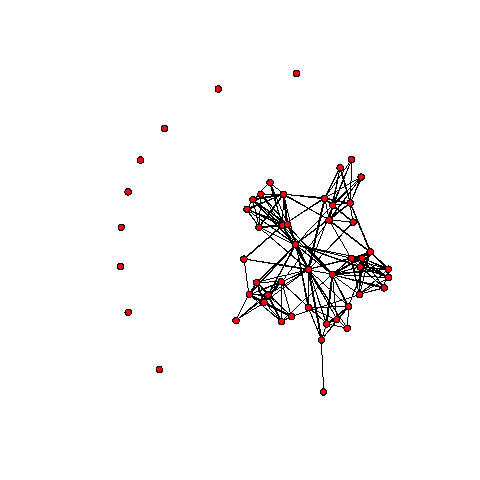
\includegraphics[scale=0.26]{pictures/m1_19_nework.png}
    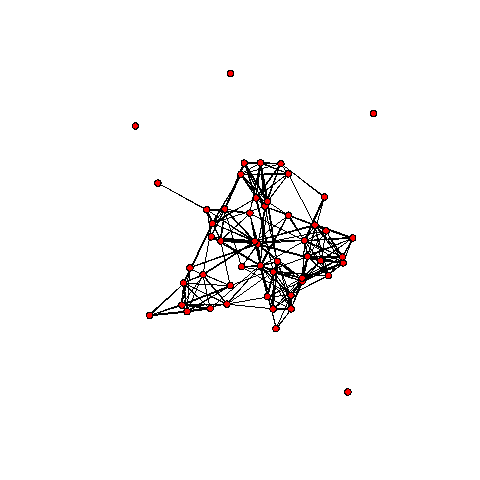
\includegraphics[scale=0.26]{pictures/w1_19_nework.png}
    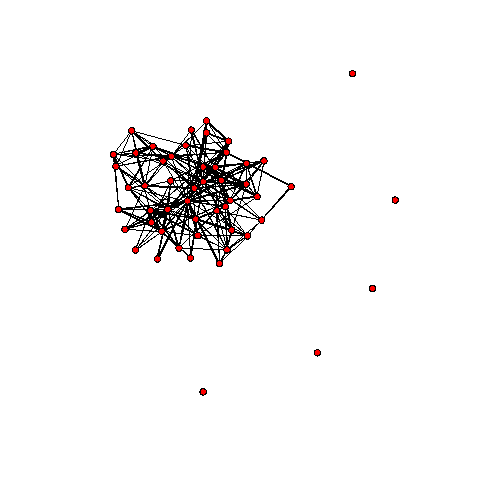
\includegraphics[scale=0.26]{pictures/f1_19_nework.png}
    \caption{Sequence 1}
    % \label{fig:ls}
    \end{center}
\end{figure}
\begin{figure}[h]
    \begin{center}
    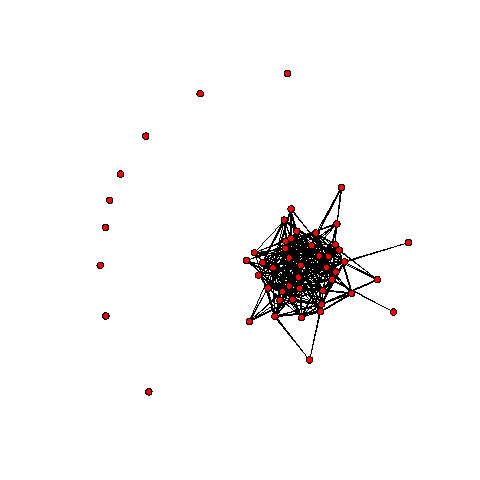
\includegraphics[scale=0.26]{pictures/m2_19_nework.png}
    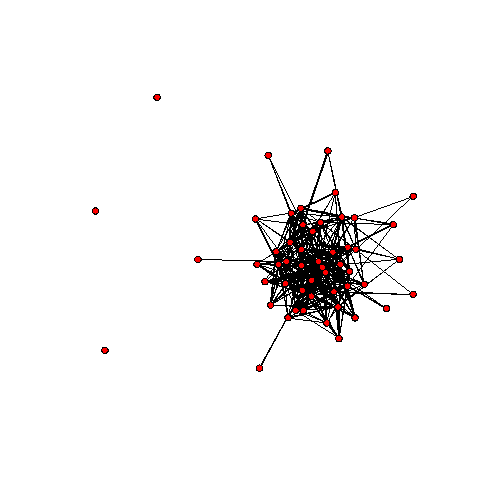
\includegraphics[scale=0.26]{pictures/w2_19_nework.png}
    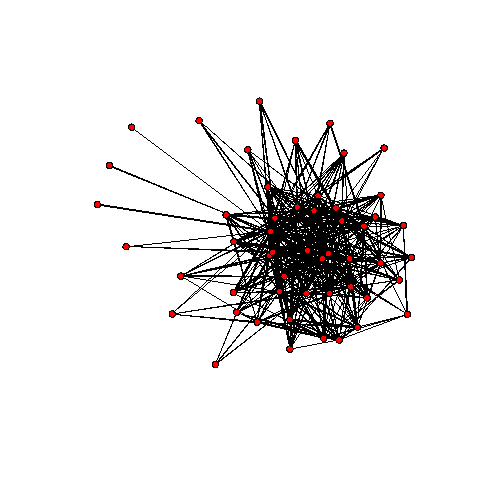
\includegraphics[scale=0.26]{pictures/f2_19_nework.png}
    \caption{Sequence 2}
    % \label{fig:ls}
    \end{center}
\end{figure}
\begin{figure}[h]
    \begin{center}
    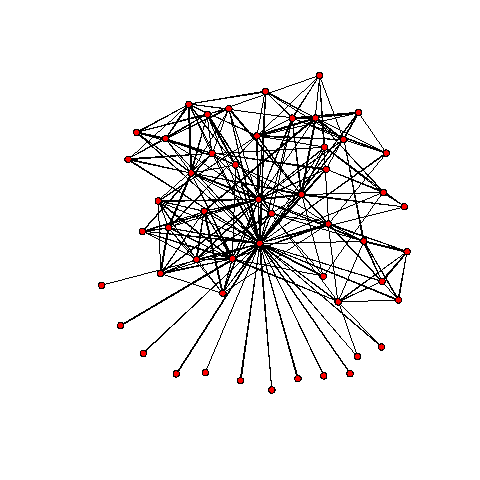
\includegraphics[scale=0.26]{pictures/m3_19_nework.png}
    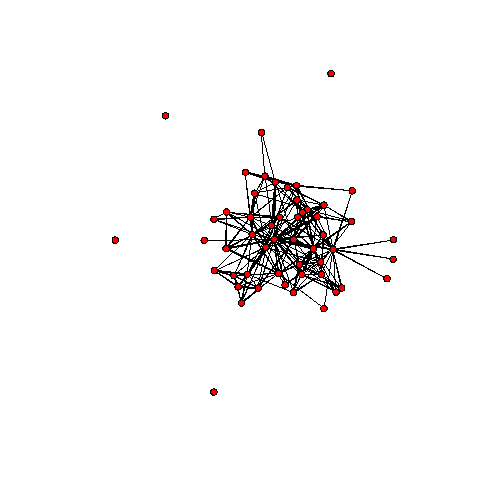
\includegraphics[scale=0.26]{pictures/w3_19_nework.png}
    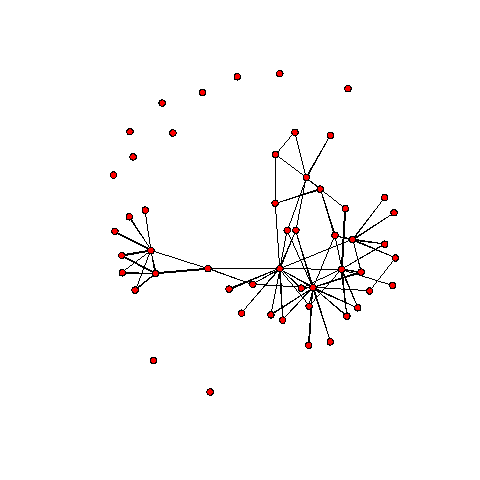
\includegraphics[scale=0.26]{pictures/f3_19_nework.png}
    \caption{Sequence 3}
    % \label{fig:ls}
    \end{center}
\end{figure}
\clearpage

I consider the 2-dimensional BSTERGM as follows.
For the formation model,
\[P(Y_t^+=y_t^+|Y_{t-1}=y_{t-1};\theta^+) = \frac{exp((\theta^+)^{T}s(y_t^+, y_{t-1}))}{c(\theta^+, y_{t-1})}\]
and for the dissolution model,
\[P(Y_t^-=y_t^-|Y_{t-1}=y_{t-1};\theta^-) = \frac{exp((\theta^-)^{T}s(y_t^-, y_{t-1}))}{c(\theta^-, y_{t-1})}\]
and by assumptions of the BSTERGMs,
\begin{align*}
    P(Y_t=y_t|Y_{t-1} &= y_{t-1};\theta^+,\theta^-)\\
    &=P(Y_t^+=y_t^+|Y_{t-1}=y_{t-1};\theta^+) P(Y_t^-=y_t^-|Y_{t-1}=y_{t-1};\theta^-)
\end{align*}
where
\(s(z_1,z_2)^T=(|z_1|-|z_2|)\)
for $z_1,z_2\in\mathcal{Y}$ with 52 nodes. In other words, the network statistic in the model is
difference of the number of edges for both the formation model and the dissolution model.

I use the ordinary normal prior $p(\theta^+)\sim\mathcal{N}(0,100)$ and $p(\theta^-)\sim\mathcal{N}(0,100)$,
and set the proposal distribution of main chain to $\epsilon\sim\mathcal{N}(0,0.0004)$.
The auxiliary chains consist of 1000 iterations, and the main chain consists of 50000 iterations.
In this setting, the BSTERGM fitting algorithm runs 2400 iterations of the main chain per minute on the intel i7-8700(3.20GHz) CPU.

After generating the chain, I cut the first 10000 samples for a burn-in period and thin the sample by 10.
The summary estimates and histograms for the posterior distributions of each parameter are as follows.

%mean, sd
\begin{table}[h!]
    \centering
        \begin{tabular}{c | c | c | c }
            Sequence & Parameter & Estimated Mean & Estimated Std.Error \\
            \hline \hline
            1 & $\theta^+$ & -2.336387 & 0.1274921 \\
            1 & $\theta^-$ & 1.043077 & 0.1722938 \\
            2 & $\theta^+$ & -1.435648 & 0.1009999 \\
            2 & $\theta^-$ & 0.9332358 & 0.1358161 \\
            3 & $\theta^+$ & -5.02916 & 0.2097569 \\
            3 & $\theta^-$ & 2.225616 & 0.1904817 \\
        \end{tabular}
        \caption{Fitted parameters summary}
        % \label{tab:data}
    \end{table}

%hist
\begin{figure}[h]
    \begin{center}
        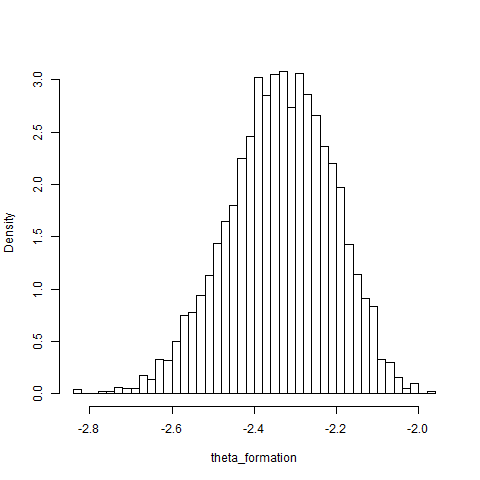
\includegraphics[scale=0.395]{pictures/net1seq_chain1_BSTERGM_formation_histogram.png}
        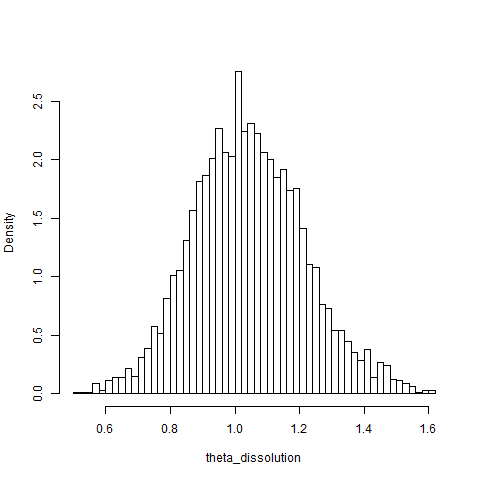
\includegraphics[scale=0.395]{pictures/net1seq_chain1_BSTERGM_dissolution_histogram.png}
    \caption{Sequence 1, posterior histogram, left: formation, right: dissolution}
    % \label{fig:ls}
    \end{center}
\end{figure}

\begin{figure}[h]
    \begin{center}
        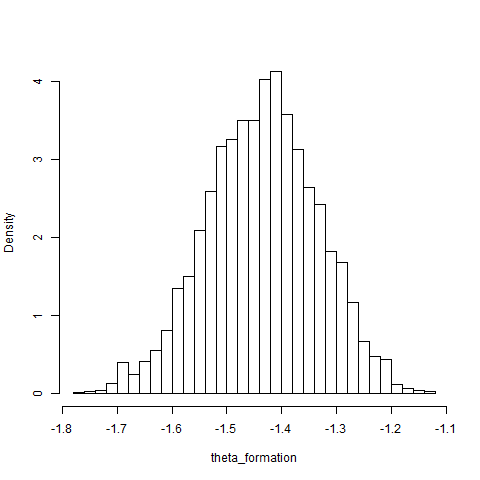
\includegraphics[scale=0.395]{pictures/net2seq_chain1_BSTERGM_formation_histogram.png}
        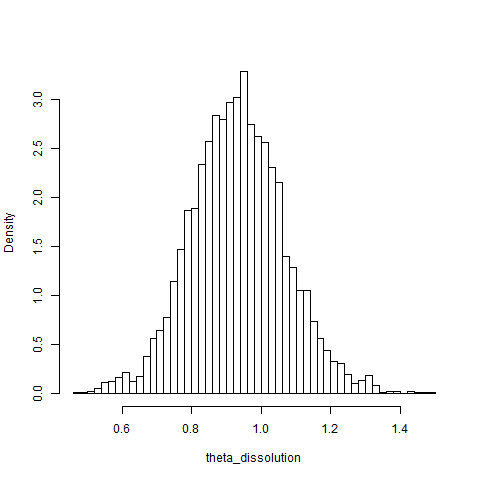
\includegraphics[scale=0.395]{pictures/net2seq_chain1_BSTERGM_dissolution_histogram.png}
    \caption{Sequence 2, posterior histogram, left: formation, right: dissolution}
    % \label{fig:ls}
    \end{center}
\end{figure}

\begin{figure}[h]
    \begin{center}
        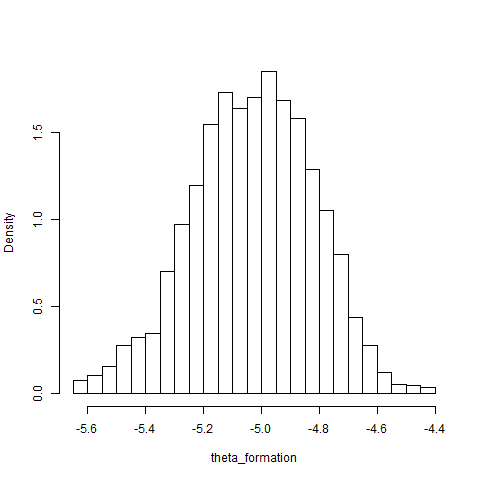
\includegraphics[scale=0.395]{pictures/net3seq_chain1_BSTERGM_formation_histogram.png}
        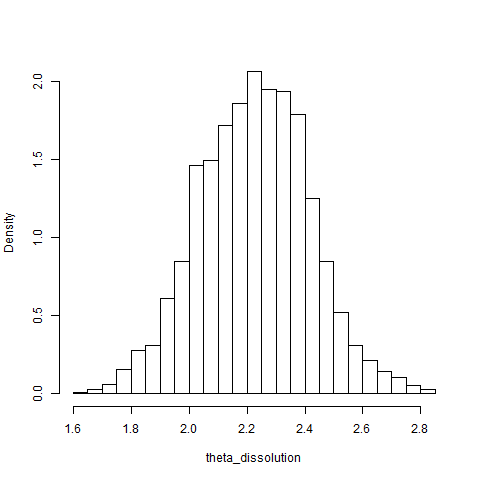
\includegraphics[scale=0.395]{pictures/net3seq_chain1_BSTERGM_dissolution_histogram.png}
    \caption{Sequence 3, posterior histogram, left: formation, right: dissolution}
    % \label{fig:ls}
    \end{center}
\end{figure}
\clearpage

For the diagnostics, I attach trace plots and autocorrelation plots.
The autocorrelation of each chain decreases rapidly as lag increases.
Moreover, trace plots show that the MCMC samples are mixed well.

\begin{figure}[h]
    \begin{center}
        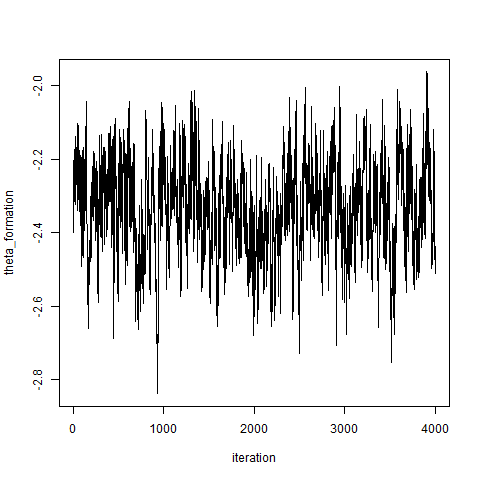
\includegraphics[scale=0.395]{pictures/net1seq_chain1_BSTERGM_formation_traceplot.png}
        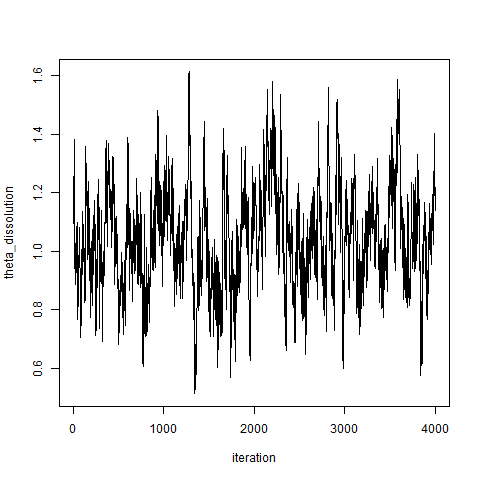
\includegraphics[scale=0.395]{pictures/net1seq_chain1_BSTERGM_dissolution_traceplot.png} \\
        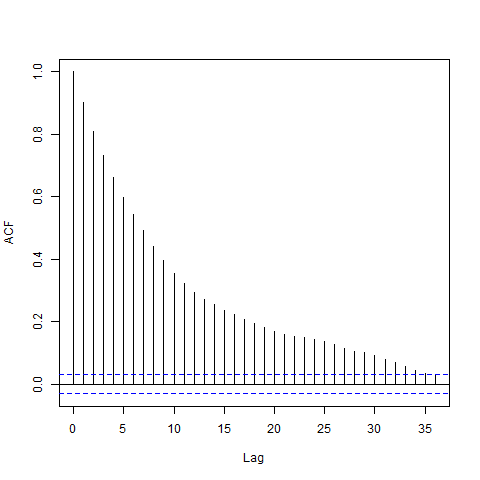
\includegraphics[scale=0.395]{pictures/net1seq_chain1_BSTERGM_formation_acf.png}
        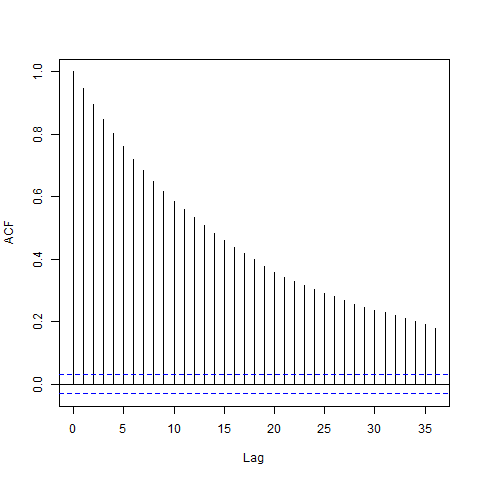
\includegraphics[scale=0.395]{pictures/net1seq_chain1_BSTERGM_dissolution_acf.png}
    \caption{Sequence 1, diagnostics plots, left: formation, right: dissolution}
    % \label{fig:ls}
    \end{center}
\end{figure}
\begin{figure}[h]
    \begin{center}
        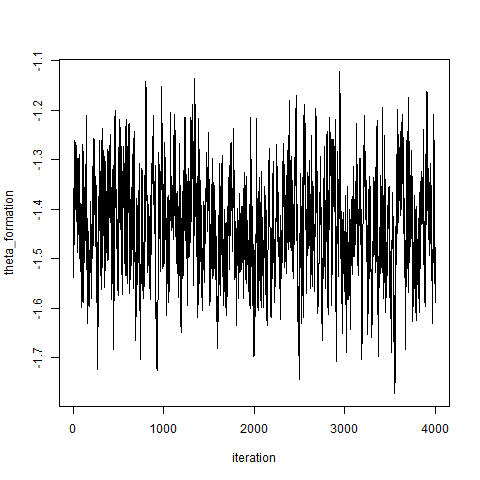
\includegraphics[scale=0.395]{pictures/net2seq_chain1_BSTERGM_formation_traceplot.png}
        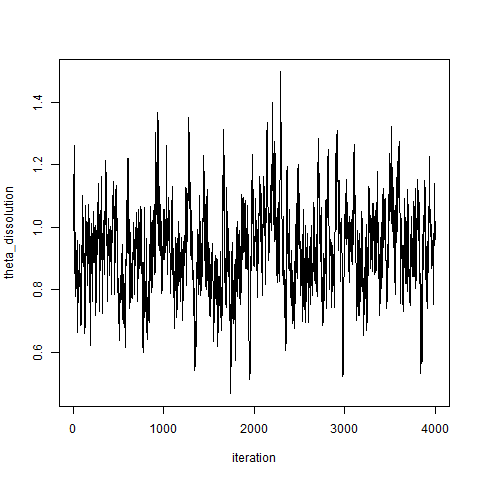
\includegraphics[scale=0.395]{pictures/net2seq_chain1_BSTERGM_dissolution_traceplot.png} \\
        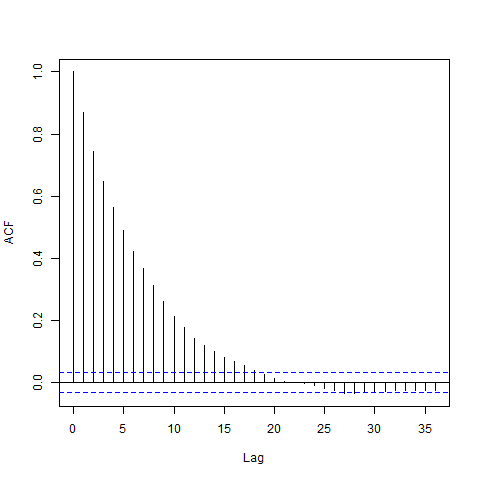
\includegraphics[scale=0.395]{pictures/net2seq_chain1_BSTERGM_formation_acf.png}
        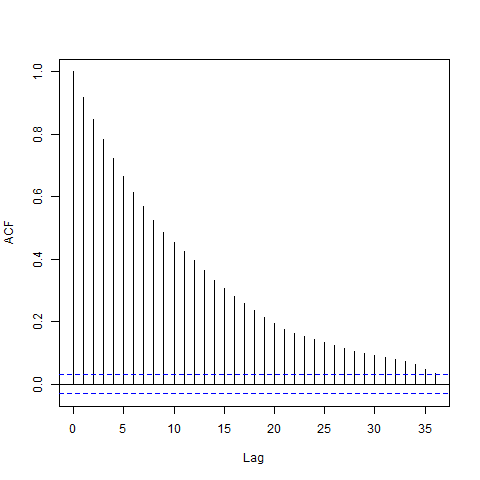
\includegraphics[scale=0.395]{pictures/net2seq_chain1_BSTERGM_dissolution_acf.png}
    \caption{Sequence 2, diagnostics plots, left: formation, right: dissolution}
    % \label{fig:ls}
    \end{center}
\end{figure}
\begin{figure}[h]
    \begin{center}
        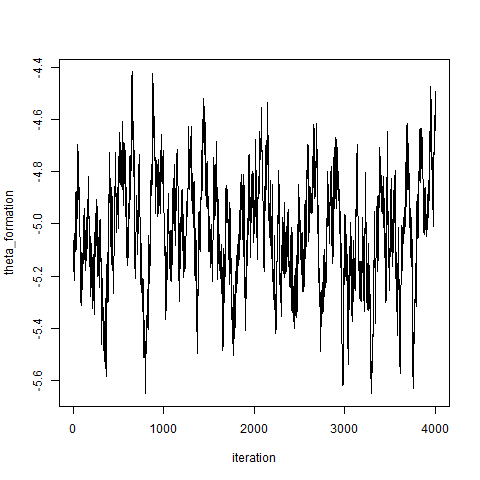
\includegraphics[scale=0.395]{pictures/net3seq_chain1_BSTERGM_formation_traceplot.png}
        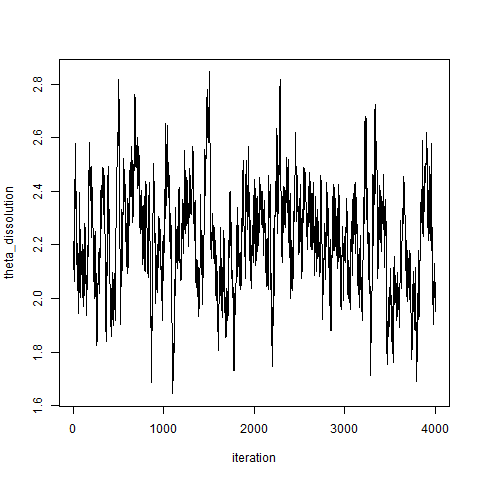
\includegraphics[scale=0.395]{pictures/net3seq_chain1_BSTERGM_dissolution_traceplot.png} \\
        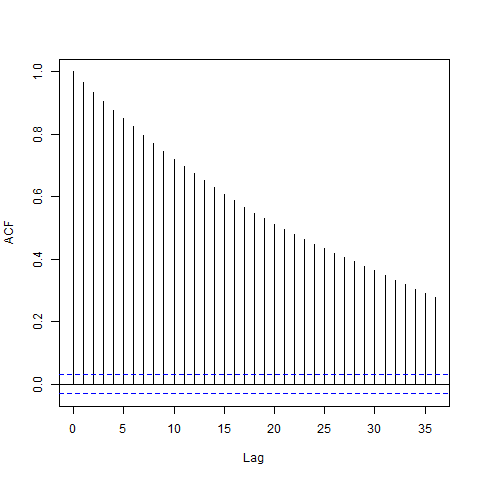
\includegraphics[scale=0.395]{pictures/net3seq_chain1_BSTERGM_formation_acf.png}
        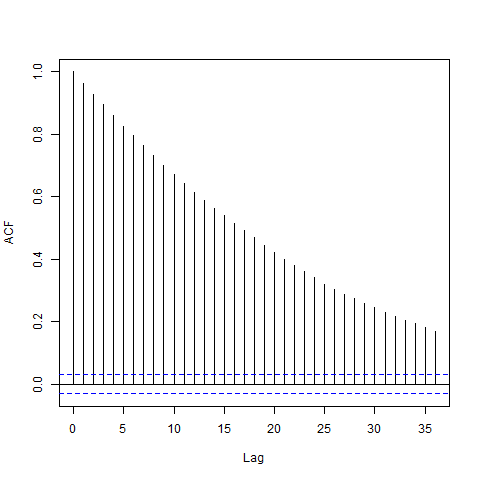
\includegraphics[scale=0.395]{pictures/net3seq_chain1_BSTERGM_dissolution_acf.png}
    \caption{Sequence 3, diagnostics plots, left: formation, right: dissolution}
    % \label{fig:ls}
    \end{center}
\end{figure}
\clearpage

In addition, as a procedure of diagnostics for auxiliary chains,
here are trace plots of the number of edges in the last auxiliary chain.
They show that all chains do not degenerate at the last parameter point during auxiliary chain iterations.

%lastsampler
\begin{figure}[h]
    \begin{center}
        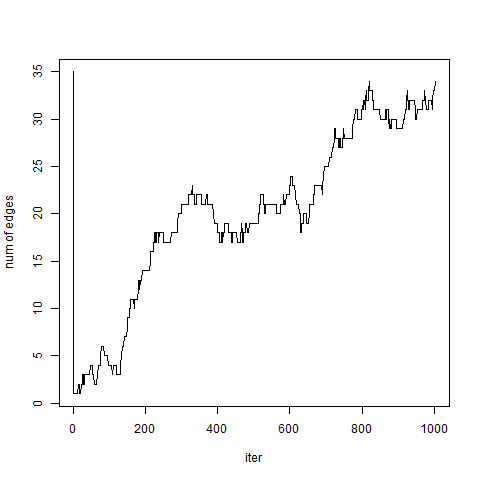
\includegraphics[scale=0.26]{pictures/net1seq_chain1_lastsampler_num_edges.png}
        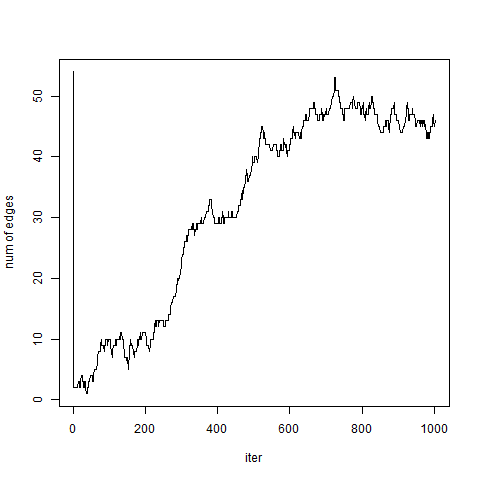
\includegraphics[scale=0.26]{pictures/net2seq_chain1_lastsampler_num_edges.png}
        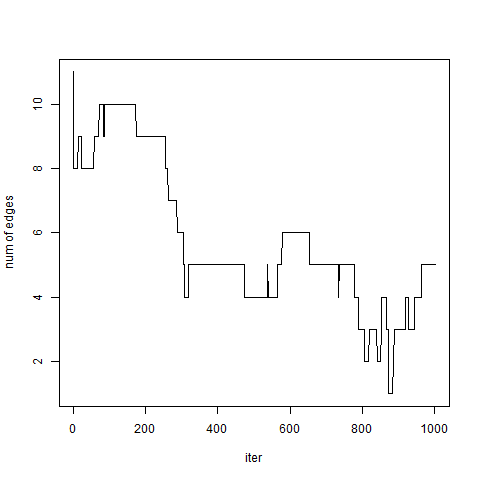
\includegraphics[scale=0.26]{pictures/net3seq_chain1_lastsampler_num_edges.png}
    \caption{The number of nodes of exchange samples in the last auxiliary chains,\\left: Sequence 1, middle: Sequence 2, right: Sequence 3}
    % \label{fig:ls}
    \end{center}
\end{figure}


Finally, I append the results of the goodness of fit check.
By comparing the observed value on the data with simulated values' quantiles generated by the goodness-of-fit algorithm,
we can check whether the fitting results are proper or not.
Some parts of sufficient statistics are selected as the network statistics in the goodness of fit procedure.
Since the example model merely has just two edge terms, 
and since the BSTERGMs share the same parameter for each network statistics but values of network statistics are different at each time point, 
the sufficient statistics do not fit perfectly to observed networks' values. 
However, the tendency of simulated values goes with the observed values.


\begin{table}[h!]
    \centering
        \begin{tabular}{c| c | c | c | c |c |c |c |c }
            Sequence& timelag & netstat & obs & q0.1 & q0.25 & q0.5 & q0.75 & q0.9 \\
            \hline \hline
            1 & 1-2 & $D_0$ & 4 &  0& 0& 0& 1& 1 \\
            1 & 1-2 & $D_1$ & 1 &  0& 0& 1& 2& 3 \\
            1 & 1-2 & $D_2$ & 0 &  1& 1& 2& 3& 4 \\
            1 & 1-2 & $D_3$ & 3 &  1& 2& 3& 4& 5 \\
            1 & 1-2 & $D_4$ & 1 &  1& 2& 3& 4& 6 \\
            1 & 1-2 & $D_5$ & 3 &  2& 3& 4& 5& 7 \\
            1 & 1-2 & $D_6$ & 3 &  2& 3& 5& 6& 8 \\
            1 & 1-2 & $D_7$ & 5 &  3& 4& 5& 7& 9 \\
            1 & 1-2 & $D_8$ & 9 &  3& 4& 6& 7& 9 \\
            1 & 1-2 & $D_9$ & 5 &  3& 4& 6& 7& 9 \\
            1 & 1-2 & $D_{10}$ & 4 &  2& 3& 5& 6& 8 \\
            1 & 1-2 & $D_{11}$ & 4 &  1& 2& 4& 5& 6 \\
            1 & 1-2 & $D_{12}$ & 4 &  0& 1& 2& 3& 5 \\
            1 & 1-2 & $D_{13}$ & 2 &  0& 1& 1& 2& 3 \\
            1 & 1-2 & $D_{14}$ & 1 &  0& 0& 1& 1& 2 \\
            1 & 1-2 & $D_{15}$ & 0 &  0& 0& 0& 1& 2 \\
            1 & 1-2 & $P_0$ & 8 &  25& 28& 33& 37& 42 \\
            1 & 1-2 & $P_1$ & 10 & 29& 33& 38& 43& 48 \\
            1 & 1-2 & $P_2$ & 29 & 30& 33& 38& 43& 47 \\
            1 & 1-2 & $P_3$ & 27 & 28& 32& 36& 40& 44 \\
            1 & 1-2 & $P_4$ & 13 & 19& 23& 28& 32& 37 \\
            1 & 1-2 & $P_5$ & 37 &  9& 13& 17& 22& 26 \\
            1 & 1-2 & $P_6$ & 40 &  3& 5& 8& 11& 15 \\
            1 & 1-2 & $P_7$ & 20 &  3& 4& 5& 7& 9 \\
            1 & 1-2 & $P_8$ & 20 &  0& 1& 3& 5& 7 \\
            1 & 1-2 & $|y_2|$ & 212 &  186& 194& 204& 214& 223 \\
        \end{tabular}
        \caption{GOF: sequence 1 (1)}
        % \label{tab:data}
    \end{table}
\clearpage
\begin{table}[h!]
    \centering
        \begin{tabular}{c| c | c | c | c |c |c |c |c }
            Sequence& timelag & netstat & obs & q0.1 & q0.25 & q0.5 & q0.75 & q0.9 \\
            \hline \hline
            1 & 2-3 & $D_0$ & 5 &  0& 0& 0& 0& 1 \\
            1 & 2-3 & $D_1$ & 0 &  0& 0& 0& 1& 2 \\
            1 & 2-3 & $D_2$ & 2 &  0& 0& 1& 2& 2 \\
            1 & 2-3 & $D_3$ & 1 &  0& 1& 2& 2& 3 \\
            1 & 2-3 & $D_4$ & 2 &  1& 1& 2& 3& 4 \\
            1 & 2-3 & $D_5$ & 5 &  1& 2& 3& 4& 5 \\
            1 & 2-3 & $D_6$ & 2 &  1& 3& 4& 5& 7 \\
            1 & 2-3 & $D_7$ & 3 &  2& 4& 5& 7& 8 \\
            1 & 2-3 & $D_8$ & 8 &  3& 4& 6& 7& 8 \\
            1 & 2-3 & $D_9$ & 4 &  3& 5& 6& 8& 9 \\
            1 & 2-3 & $D_{10}$ & 4 &  3& 4& 5& 7& 9 \\
            1 & 2-3 & $D_{11}$ & 5 &  2& 3& 5& 6& 8 \\
            1 & 2-3 & $D_{12}$ & 1 &  1& 2& 4& 5& 6 \\
            1 & 2-3 & $D_{13}$ & 3 &  1& 2& 2& 4& 5 \\
            1 & 2-3 & $D_{14}$ & 0 &  0& 1& 2& 3& 4 \\
            1 & 2-3 & $D_{15}$ & 1 &  0& 0& 1& 2& 3 \\
            1 & 2-3 & $P_0$ & 11 & 20& 24& 28& 32& 37 \\
            1 & 2-3 & $P_1$ & 12 & 32& 36& 41& 47& 51 \\
            1 & 2-3 & $P_2$ & 23 & 35& 39& 44& 49& 53 \\
            1 & 2-3 & $P_3$ & 52 & 32& 35& 40& 45& 49 \\
            1 & 2-3 & $P_4$ & 39 & 24& 28& 33& 37& 42 \\
            1 & 2-3 & $P_5$ & 24 & 13& 18& 22& 27& 32 \\
            1 & 2-3 & $P_6$ & 21 &  6& 9& 12& 17& 21 \\
            1 & 2-3 & $P_7$ & 20 &  2& 3& 5& 8& 12 \\
            1 & 2-3 & $P_8$ & 13 &  0& 1& 2& 4& 6 \\
            1 & 2-3 & $|y_3|$ & 227 &  213& 222& 232& 243& 253 \\
        \end{tabular}
        \caption{GOF: sequence 1 (2)}
        % \label{tab:data}
    \end{table}
\clearpage

\begin{table}[h!]
    \centering
        \begin{tabular}{c| c | c | c | c |c |c |c |c }
            Sequence& timelag & netstat & obs & q0.1 & q0.25 & q0.5 & q0.75 & q0.9 \\
            \hline \hline
            2 & 1-2 & $D_0$ & 3 &  0& 0& 0& 0& 0 \\
            2 & 1-2 & $D_1$ & 2 &  0& 0& 0& 0& 0 \\
            2 & 1-2 & $D_2$ & 4 &  0& 0& 0& 0& 1 \\
            2 & 1-2 & $D_3$ & 1 &  0& 0& 0& 1& 1 \\
            2 & 1-2 & $D_4$ & 3 &  0& 0& 1& 1& 2 \\
            2 & 1-2 & $D_5$ & 0 &  0& 0& 1& 2& 3 \\
            2 & 1-2 & $D_6$ & 0 &  0& 1& 2& 3& 4 \\
            2 & 1-2 & $D_7$ & 1 &  0& 1& 2& 3& 4 \\
            2 & 1-2 & $D_8$ & 4 &  1& 1& 2& 4& 5 \\
            2 & 1-2 & $D_9$ & 1 &  1& 1& 2& 3& 5 \\
            2 & 1-2 & $D_{10}$ & 3 &  1& 2& 3& 4& 5 \\
            2 & 1-2 & $D_{11}$ & 1 &  1& 2& 2& 4& 5 \\
            2 & 1-2 & $D_{12}$ & 1 &  1& 2& 3& 4& 5 \\
            2 & 1-2 & $D_{13}$ & 2 &  1& 2& 3& 4& 5 \\
            2 & 1-2 & $D_{14}$ & 3 &  1& 2& 3& 4& 5 \\
            2 & 1-2 & $D_{15}$ & 1 &  1& 2& 3& 4& 6 \\
            2 & 1-2 & $D_{16}$ & 1 &  1& 2& 3& 4& 6 \\
            2 & 1-2 & $D_{17}$ & 3 &  1& 2& 2& 4& 6 \\
            2 & 1-2 & $D_{18}$ & 2 &  1& 2& 3& 4& 6 \\
            2 & 1-2 & $D_{19}$ & 2 &  1& 2& 3& 4& 5 \\
            2 & 1-2 & $D_{20}$ & 2 &  1& 2& 3& 4& 5 \\
            2 & 1-2 & $D_{21}$ & 2 &  0& 1& 2& 3& 4 \\
            2 & 1-2 & $P_4$ & 21 & 33& 38& 43& 48& 52 \\
            2 & 1-2 & $P_5$ & 28 & 35& 38& 43& 48& 54 \\
            2 & 1-2 & $P_6$ & 31 & 33& 37& 42& 47& 52 \\
            2 & 1-2 & $P_7$ & 31 & 28& 32& 37& 43& 48 \\
            2 & 1-2 & $P_8$ & 32 & 21& 25& 31& 36& 41 \\
            2 & 1-2 & $P_9$ & 23 & 14& 18& 23& 29& 33 \\
            2 & 1-2 & $P_{10}$ & 27 & 8& 12& 16& 21& 26 \\
            2 & 1-2 & $P_{11}$ & 21 & 4& 7& 10& 14& 19 \\
            2 & 1-2 & $|y_2|$ & 342 &  344& 356& 370& 387& 400 \\
        \end{tabular}
        \caption{GOF: sequence 2 (1)}
        % \label{tab:data}
    \end{table}
\clearpage
\begin{table}[h!]
    \centering
        \begin{tabular}{c| c | c | c | c |c |c |c |c }
            Sequence& timelag & netstat & obs & q0.1 & q0.25 & q0.5 & q0.75 & q0.9 \\
            \hline \hline
            2 & 2-3 & $D_0$ & 0 &  0& 0& 0& 0& 0 \\
            2 & 2-3 & $D_1$ & 3 &  0& 0& 0& 0& 0 \\
            2 & 2-3 & $D_2$ & 1 &  0& 0& 0& 0& 0 \\
            2 & 2-3 & $D_3$ & 2 &  0& 0& 0& 0& 1 \\
            2 & 2-3 & $D_4$ & 2 &  0& 0& 0& 1& 2 \\
            2 & 2-3 & $D_5$ & 1 &  0& 0& 1& 1& 2 \\
            2 & 2-3 & $D_6$ & 1 &  0& 0& 1& 2& 3 \\
            2 & 2-3 & $D_7$ & 2 &  0& 1& 2& 3& 4 \\
            2 & 2-3 & $D_8$ & 1 &  1& 1& 2& 3& 4 \\
            2 & 2-3 & $D_9$ & 1 &  1& 1& 2& 3& 5 \\
            2 & 2-3 & $D_{10}$ & 3 &  1& 2& 3& 4& 5 \\
            2 & 2-3 & $D_{11}$ & 2 &  1& 1& 2& 4& 5 \\
            2 & 2-3 & $D_{12}$ & 2 &  1& 2& 4& 5& 6 \\
            2 & 2-3 & $D_{13}$ & 3 &  1& 2& 3& 4& 5 \\
            2 & 2-3 & $D_{14}$ & 2 &  1& 2& 3& 4& 5 \\
            2 & 2-3 & $D_{15}$ & 0 &  1& 2& 3& 4& 5 \\
            2 & 2-3 & $D_{16}$ & 3 &  1& 2& 3& 4& 5 \\
            2 & 2-3 & $D_{17}$ & 1 &  1& 2& 2& 4& 5 \\
            2 & 2-3 & $D_{18}$ & 0 &  1& 2& 3& 4& 5 \\
            2 & 2-3 & $D_{19}$ & 3 &  1& 2& 3& 4& 5 \\
            2 & 2-3 & $D_{20}$ & 2 &  1& 2& 3& 4& 5 \\
            2 & 2-3 & $D_{21}$ & 0 &  1& 1& 2& 3& 4 \\
            2 & 2-3 & $P_4$ & 6 & 35& 29& 44& 48& 53 \\
            2 & 2-3 & $P_5$ & 27 & 34& 38& 42& 48& 53 \\
            2 & 2-3 & $P_6$ & 34 & 35& 39& 44& 49& 53 \\
            2 & 2-3 & $P_7$ & 25 & 33& 36& 41& 46& 50 \\
            2 & 2-3 & $P_8$ & 27 & 28& 32& 27& 42& 47 \\
            2 & 2-3 & $P_9$ & 39 & 22& 26& 31& 36& 40 \\
            2 & 2-3 & $P_{10}$ & 24 & 15& 19& 24& 29& 34 \\
            2 & 2-3 & $P_{11}$ & 27 & 10& 14& 18& 23& 27 \\
            2 & 2-3 & $|y_3|$ & 433 &  375& 387& 402& 417& 430 \\
        \end{tabular}
        \caption{GOF: sequence 2 (2)}
        % \label{tab:data}
    \end{table}
\clearpage


\begin{table}[h!]
    \centering
        \begin{tabular}{c| c | c | c | c |c |c |c |c }
            Sequence& timelag & netstat & obs & q0.1 & q0.25 & q0.5 & q0.75 & q0.9 \\
            \hline \hline
            3 & 1-2 & $D_0$ & 4 &  0& 0& 0& 1& 2 \\
            3 & 1-2 & $D_1$ & 4 &  6& 7& 8& 9& 10 \\
            3 & 1-2 & $D_2$ & 3 &  1& 2& 3& 4& 5 \\
            3 & 1-2 & $D_3$ & 1 &  0& 0& 1& 1& 2 \\
            3 & 1-2 & $D_4$ & 2 &  0& 1& 1& 2& 3 \\
            3 & 1-2 & $D_5$ & 7 &  1& 2& 3& 4& 5 \\
            3 & 1-2 & $D_6$ & 4 &  3& 4& 5& 7& 8 \\
            3 & 1-2 & $D_7$ & 3 &  3& 4& 5& 6& 7 \\
            3 & 1-2 & $D_8$ & 4 &  2& 3& 4& 5& 6 \\
            3 & 1-2 & $D_9$ & 6 &  2& 3& 4& 5& 6 \\
            3 & 1-2 & $D_{10}$ & 0 &  2& 3& 4& 5& 6 \\
            3 & 1-2 & $D_{11}$ & 6 &  2& 3& 4& 5& 6 \\
            3 & 1-2 & $D_{12}$ & 2 &  1& 1& 2& 3& 4 \\
            3 & 1-2 & $D_{13}$ & 1 &  0& 1& 1& 2& 3 \\
            3 & 1-2 & $D_{14}$ & 0 &  0& 1& 1& 2& 3 \\
            3 & 1-2 & $D_{15}$ & 0 &  0& 0& 1& 1& 2 \\
            3 & 1-2 & $P_0$ & 7 & 9& 10& 12& 13& 14 \\
            3 & 1-2 & $P_1$ & 22 & 12& 14& 17& 20& 23 \\
            3 & 1-2 & $P_2$ & 21 & 15& 18& 21& 24& 27 \\
            3 & 1-2 & $P_3$ & 42 & 23& 27& 30& 34& 37 \\
            3 & 1-2 & $P_4$ & 24 & 25& 29& 32& 36& 40 \\
            3 & 1-2 & $P_5$ & 32 & 22& 25& 29& 33& 37 \\
            3 & 1-2 & $P_6$ & 14 & 15& 18& 21& 23& 26 \\
            3 & 1-2 & $P_7$ & 9 & 12& 14& 17& 19& 22 \\
            3 & 1-2 & $P_8$ & 14 & 7& 9& 12& 14& 16 \\
            3 & 1-2 & $P_9$ & 6 &  3& 5& 7& 9& 11 \\
            3 & 1-2 & $P_10$ & 1 &  1& 2& 3& 4& 5 \\
            3 & 1-2 & $|y_2|$ & 196 &  198& 201& 206& 209& 213 \\
        \end{tabular}
        \caption{GOF: sequence 3 (1)}
        % \label{tab:data}
    \end{table}
\clearpage
\begin{table}[h!]
    \centering
        \begin{tabular}{c| c | c | c | c |c |c |c |c }
            Sequence& timelag & netstat & obs & q0.1 & q0.25 & q0.5 & q0.75 & q0.9 \\
            \hline \hline
            3 & 2-3 & $D_0$ & 11 &  2& 3& 3& 4& 4 \\
            3 & 2-3 & $D_1$ & 11 &  2& 3& 4& 5& 6 \\
            3 & 2-3 & $D_2$ & 12 &  2& 2& 3& 4& 5 \\
            3 & 2-3 & $D_3$ & 9 &  1& 1& 2& 3& 3 \\
            3 & 2-3 & $D_4$ & 2 &  2& 2& 3& 4& 5 \\
            3 & 2-3 & $D_5$ & 1 &  4& 5& 6& 7& 8 \\
            3 & 2-3 & $D_6$ & 0 &  2& 3& 4& 6& 7 \\
            3 & 2-3 & $D_7$ & 2 &  2& 3& 4& 5& 6 \\
            3 & 2-3 & $D_8$ & 1 &  2& 3& 4& 5& 6 \\
            3 & 2-3 & $D_9$ & 0 &  2& 3& 4& 5& 6 \\
            3 & 2-3 & $D_{10}$ & 1 &  1& 2& 3& 4& 5 \\
            3 & 2-3 & $D_{11}$ & 0 &  1& 2& 3& 4& 5 \\
            3 & 2-3 & $D_{12}$ & 0 &  0& 1& 1& 2& 3 \\
            3 & 2-3 & $D_{13}$ & 0 &  0& 0& 0& 1& 2 \\
            3 & 2-3 & $D_{14}$ & 1 &  0& 0& 0& 0& 1 \\
            3 & 2-3 & $D_{15}$ & 1 &  0& 0& 0& 1& 1 \\
            3 & 2-3 & $P_0$ & 36 & 8& 10& 12& 14& 16 \\
            3 & 2-3 & $P_1$ & 26 & 20& 22& 25& 28& 31 \\
            3 & 2-3 & $P_2$ & 4 & 23& 26& 30& 34& 37 \\
            3 & 2-3 & $P_3$ & 0 & 29& 33& 37& 40& 44 \\
            3 & 2-3 & $P_4$ & 1 & 21& 24& 27& 31& 34 \\
            3 & 2-3 & $P_5$ & 0 & 16& 18& 22& 25& 28 \\
            3 & 2-3 & $P_6$ & 0 &  8& 10& 12& 14& 16 \\
            3 & 2-3 & $P_7$ & 1 &  6& 7& 9& 11& 13 \\
            3 & 2-3 & $P_8$ & 0 &  3& 4& 6& 8& 10 \\
            3 & 2-3 & $P_9$ & 0 &  1& 1& 2& 4& 5 \\
            3 & 2-3 & $P_10$ & 0 &  0& 1& 1& 2& 3 \\
            3 & 2-3 & $|y_3|$ & 227 &  180& 183& 187& 190& 193 \\
        \end{tabular}
        \caption{GOF: sequence 3 (2)}
        % \label{tab:data}
    \end{table}
\clearpage


%--------------------------------------------------------------------------------%
%--------------------------------------------------------------------------------%
\chapter{Summary and Discussion}\label{Chapter7}
\section{Summary and discussion}

In this paper, I have proposed the Bayesian STERGMs for statistical analysis on a sequence of networks. 
I also provide the algorithm to estimate the model's parameters and the inference method 
following the standard Bayesian approach. 
Moreover, an application to real data is shown using BSTERGMs.

Since the BSTERGMs have their base on the ERGMs, the models are flexible and can include various network statistics. 
Moreover, the BSTERGMs can be applied to more general networks, including weighted graphs. 
Moreover, by combining these features, the BSTERGM can take the weights as covariates of the model
by a little of modification as the ERGM can.

On the other hand, since the BSTERGMs are using the exchange algorithm, 
the models can be integrated with other methods to help the MCMC chains to converge and run faster. 
For example, the 'tie no tie'(TNT) algorithm used by ergm package (\cite{RN100}) can be applied 
to enhance the performance of the auxiliary chain of the BSTERGMs.

Modeling by the BSTERGMs for large networks is possible, 
but a problem of computational inefficiency rises. 
If the observed networks in the given sequence have lots of nodes, 
the estimation algorithm for the BSTERGM needs a vast number of iterations in the auxiliary chains 
to draw a proper exchange sample at a given parameter point. 
In addition, the calculation of network statistics in the model causes another problem for large networks, 
especially when the network statistics demand computation with high complexity.
For example, calculating the edgewise shared partner distribution of one network 
needs computation of complexity $O(n^3)$, 
so computation cost increases rapidly as the number of nodes $n$ grows, and 
the calculating $\pi$ may become bottlenecks of the whole computation procedure.

Another critical issue related to the BSTERGMs is degeneracy. 
As I have mentioned in chapter 5, 
the convergence of BSTERGMs fitting algorithm is very sensitive to the main MCMC chain's initial point, 
so searching a region for non-degenerate initial parameter point in the parameter space is very important. 
Often, however, finding the region is tricky work for the BSTERGMs, partly because there are too many parameters. 
Since the BSTERGMs have two parts - a formation model and a dissolution model - in the setting of the models by definition, 
the dimension of the parameter space tends to increase 
although each formation and dissolution model does not have too many terms, respectively. 
What makes the situation worse is not only the high dimension of parameter space but also the shape of the convergent region in the space. 
In many cases, the region is geometrically curved 
due to an implicit relation between several network statistics in the models and interaction between the formation model and dissolution model. 
Then, the fitting algorithm's main chain may fail to explore the whole parameter space.
As a result, the fitting algorithm suffers a non-convergence problem. 
Imposing some model level constraint or using a special prior may be a remedy, 
but finding the proper constraint or the prior distribution will often be a more difficult problem than the original one. 
Thus, further research is needed to resolve these issues.


\section{Supplements}
You can find the C++ implementation (using Armadilo: see http://arma.sourceforge.net/)
of the BSTERGM fitting, diagnostic, and GOF algorithms
at my Github page: \\
https://github.com/letsjdosth/BayesianSTERGM.




%--------------------------------------------------------------------------------%
%--------------------------------------------------------------------------------%


%--------------------------------------------------------------------------------%
%--------------------------------------------------------------------------------%




%--------------------------------------------------------------------------------%
%--------------------------------------------------------------------------------%



%--------------------------------------------------------------------------------%
%--------------------------------------------------------------------------------%


%--------------------------------------------------------------------------------%
%--------------------------------------------------------------------------------%




\nocite{*}
\bibliographystyle{apalike}
\bibliography{paper_format}



% %----------------------------------------------------------
\newpage

\section*{국문 초록}
\setstretch{1.8}
\par
\bigskip

\begin{center}
\large
BSTERGMs: 베이지안 분해 가능-시간 지수 랜덤 그래프 모형 
\end{center}
\setstretch{1.8}
\par
\bigskip
\noindent
분해 가능-시간 지수 랜덤 그래프 모형(STERGMs)은 시간에 따라 변화하는
동적 네트워크의 구조 변화를 묘사하는 데에 유용한 모형이나,
이 모형에 대한 베이지안 접근은 지금까지 이루어지지 않았었다.
이 논문에서는, STERGMs에 대한 베이즈 통계학적 접근인 베이지안 분해 가능-시간 지수 랜덤 그래프 모형(BSTERGMs)을 제안하고,
이중적으로 추적 불가능한 정규화 상수 문제를 고려하며 사후 분포로부터 표본을 얻는
계산 알고리즘을 설명한다. 나아가, 이 모형에 대해 베이지안 방법을 통한 통계적 추론 과정을 보인다.


\bigskip
\noindent \hrulefill\\
핵심 용어 :  \par 네트워크, 지수 랜덤 그래프 모형, 베이지안 추론, 마르코프 연쇄 몬테 카를로, 시간 데이터

%\pagebreak

\newpage

% %--------------------------------------------------------------------------------%
% %--------------------------------------------------------------------------------%


\end{document}
